\documentclass[12pt]{article}
\usepackage[spanish]{babel}
\usepackage{amsmath}
\usepackage{graphicx}
\usepackage{url}
\usepackage{fancyhdr}
\pagestyle{fancy}
\usepackage{hyperref}
\usepackage{listings}

\begin{document}

\begin{center}
\bf{\sc\Huge Proyecto de investigación interrupciones}\\
\end{center}
\vspace{60pt}
\begin{center}
\bf{\sc\Huge universidad de Antioquia}\\
\end{center}
\vspace{120pt}
\begin{center}
\bf{\sc\Huge Juan Guillermo Quevedo Cifuentes }\\
\end{center}
\vspace{120pt}
\begin{center}
\bf{\sc\Huge Facultad de ingeniería}
\end{center}
\vspace{5pt}
\begin{center}
\bf{\sc\Huge Informatica II}
\end{center}
\vspace{5pt}
\begin{center}
\bf{\sc\Huge 2020}\\
\end{center}
\newpage

Cuando se utiliza hardware se puede tener la necesidad de vigilar algún periférico para ejecutar alguna instrucción, pero ¿cómo lo podemos lograr esto? Ya que, si se implementa dentro del código que se ejecuta se tendría que parar el código cíclicamente para revisar la señal del periférico, esto le cuesta tiempo al programa que podría utilizar en ejecutar las otras instrucciones. Hay una solución para este problema que son las interrupciones, lo que hacen es pausar el programa que está ejecutando, se realiza las instrucciones que el periférico requiera y cuando termine de ejecutar estas instrucciones reanudara las instrucciones interrumpidas por la señal del periférico. Las interrupciones no solo se utilizan en el hardware también se utilizan en el software, esto ya que en ocasiones se necesita recolectar información del disco duro, entonces se realiza una interrupción por software para ejecutar las instrucciones necesarias para recolectar dicha información.\cite{Sistemasintegrados}

\vspace{10}

Antes de las interrupciones se utilizaba el sondeo, es la manera simple para resolver el problema, que es que el microprocesador le pregunte constantemente al periférico que, si necesita su atención, pero este método era ineficiente ya que gastaba tiempo y capacidad del microprocesador que se podrían estar siendo usadas por las instrucciones, además que entre más periféricos controle el microprocesador mas tiempo va a mal gastar el procesador en preguntarle si necesita ser usado. Al ver este problema se idearon las interrupciones que permiten que no sea el procesador el que le pregunte al periférico si necesita su atención, si no, que el periférico sea el que le pide al microprocesador que le preste atención.\cite{interruptsmadeeasy}

\vspace{10}

Aunque se ha usado mucho el ejemplo con periféricos, las interrupciones por hardware no son las únicas que existen, ya que hay 3 tipos de interrupciones por hardware, por software y excepciones, las ultimas dos aunque se parecen no son lo mismas, porque la excepciones son causadas por un error del programa, como dividir por cero o entrar a una zona prohibida de la memoria y las interrupciones por software son cuando se necesita una función del sistema operativo, por ejemplo, entonces este interrumpe el programa virtualmente para ejecutar esta función y que al finalizar la el programa vuelva a reanudar las instrucciones interrumpidas.\cite{microprocesadoresUNAD}

\vspace{10}

Las interrupciones de hardware se logran de la siguiente manera, se reserva un espacio de memoria para almacenar las instrucciones a ejecutar cuando ocurra una interrupción, y al recibir una señal especifica por el pin que activa la interrupción el microprocesador pausa el flujo de instrucciones actuales para dirigirse a la dirección de memoria dada, ejecuta las instrucciones que encuentra allí y al terminarlas reanuda las que dejo el pausa. Las interrupciones por hardware pueden ser de dos tipos mascarables y no mascarables, lo que significa es que si la interrupción es mascarable puede ser ignorada, la decisión de ignorar la interrupción puede se tanto del sistema como del usuario, en cambio las no mascarables son interrupciones que no se pueden ignorar.

\vspace{10}

Las interrupciones por software se dan por una instrucción intencional, la forma de pedir esta interrupción varia dependiendo del hardware usado, ya que dependiendo de este varia la sintaxis que se va a utilizar en el lenguaje que se programe.

\vspace{10}

Lo siguiente es un ejemplo de interrupción en la plataforma Arduino, el objetivo de este ejemplo es demostrar las ventajas de las interrupciones y demostrar su utilidad. El proyecto consiste en 6 leds, un sensor de proximidad (este puede ser de cualquiera, hasta un pulsador) y una placa Arduino uno. El proyecto consiste en tener los leds en línea encendiendo secuencialmente y cuando el sensor detecte movimiento encenderá todos los leds al mismo tiempo por 10 segundos, para después continuar con la secuencia de los leds. Para la parte del sensor se utilizará una interrupción, ¿Por qué? Porque si se hace con sondeo el sensor de movimiento solo se reportara que esta activo cuando termine la secuencia de leds, causando retrasos o hasta puede que no se active cuando exista algún movimiento que lo debería activar. A continuación se encuentra el esquema de conexiones (Figura 1) y el código del ejemplo.

\vspace{10}

\begin{lstlisting}[language=C++]
int leds[6]={13,12,11,10,9,8};
void setup() {
  for(int i=0;i<6;i++){
    pinMode(leds[i],OUTPUT);
    digitalWrite(leds[i],LOW);}
  attachInterrupt(digitalPinToInterrupt(2),interrupcion,RISING);
  }
void interrupcion(){
  for(int i=0;i<6;i++) digitalWrite(leds[i],HIGH);
  delay(10000);
  for(int i=0;i<6;i++) digitalWrite(leds[i],LOW);
  }
void loop() {
  for(int i=0;i<6;i++){
    digitalWrite(leds[i],HIGH);
    delay(200);
    digitalWrite(leds[i],LOW);}
  for(int i=5;i>=0;i--){
    digitalWrite(leds[i],HIGH);
    delay(50);
    digitalWrite(leds[i],LOW);}
}
\end{lstlisting}

\begin{figure}[h]
    \centering
    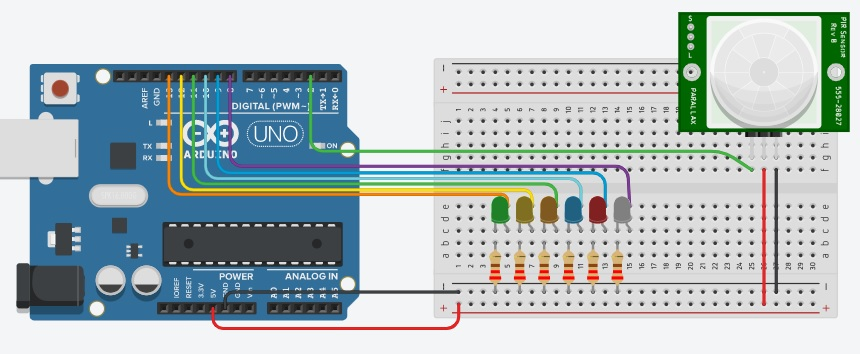
\includegraphics[width=16cm]{ejemplo.jpg}
    \caption{Ejemplo}
    \label{fig:my_label}
\end{figure}

\vspace{10}
Link de la simulación del circuito en Tinkercad: \url{https://www.tinkercad.com/things/cf15Hqa07Cu}


\newpage

\bibliographystyle{plain} 

\bibliography{Bibliografia.bib}

\end{document}

